
\documentclass[preprint,12pt]{elsarticle}

\usepackage[spanish]{babel}
\usepackage{amssymb}
\usepackage{graphicx}
\usepackage{lineno}
\usepackage[utf8]{inputenc}
\usepackage{url}
\usepackage{natbib}

\begin{document}
	
	\begin{frontmatter}

		\title{\huge COMPARATIVA DE RAPIDEZ Y SIMPLICIDAD DE USO DE UN DATAWAREHOUSE Y DATALAKE}
		
		\author{Balaguer Valles, Angela Lessly               (2016054494)}
		\author{Huallpa Castro, Leydi Katherine	      (2015053230)}
		\author{Pilco Quispe, Mireya Flavia		      (2015053234)}
		\author{Salamanca Contreras, Fiorella Rosmery (2015053237)}
		
		\address{Tacna, Perú}
		
		\begin{abstract}
			%% Text of abstract
The discussion Data Lake vs. Data Warehouse is something very common among those companies that are preparing to implement big data solutions. Quickly the conversation about data and analysis in the big data field takes us to the Data Lake or data lake, but very often the companies do not quite understand what this means and what are the differences between Data Lake vs. Data Warehouse.
		\end{abstract}
\end{frontmatter}
%%
	%% Start line numbering here if you want
	%%
	%\linenumbers
	
	%% main text
	\section{Resumen}

La discusión Data Lake vs Data Warehouse es algo muy común entre aquellas empresas que se disponen a implantar soluciones de big data. Rápidamente la conversación sobre datos y análisis en el ámbito de big data nos lleva al Data Lake o lago de datos, pero muy a menudo las empresas no acaban de entender bien qué es lo que esto significa y cuáles son las diferencias entre Data Lake vs Data Warehouse.

	%%
	%% Start line numbering here if you want
	%%
	%\linenumbers
	
	%% main text
\section{Introduccion}
Actualmente trabajar con cantidades enormes de datos empieza a ser la norma más que la excepción y, es cada vez más necesario buscar una solución más eficiente para almacenar y procesar grandes volúmenes de información.

El enfoque tradicional del DataWarehouse/Business Intelligence ha hecho un gran trabajo para simplificar el acceso a los datos y la presentación de informes, permitiendo combinar datos de muchas fuentes, con el fin de responder a las preguntas que una organización puede tener.

Los datos son la clave para entender los patrones de tus clientes, competidores y mercados. Sólo mediante el análisis de esta información se pueden tomar decisiones y llevar a cabo las acciones adecuadas.

Por ello, el reto para muchas de las compañías actuales es Integrar, Gestionar y Distribuir sus datos a aquellos que los necesitan en el menor tiempo posible, apareciendo en los últimos años el concepto de Data Lake.

	%%
	%% Start line numbering here if you want
	%%
	%\linenumbers
	
	%% main text

\section{Objetivo}
		\begin{itemize}
		\item Objetivo 1:
		\item Objetivo 2: 
		\item Objetivo 3: 

	\end{itemize}

	%%
	%% Start line numbering here if you want
	%%
	%\linenumbers
	
	%% main text

\section{Marco Teorico}
	
\subsection{DATA WAREHOUSE}	

Los profesionales en este ámbito seguro que conocen este término y, cuando se empieza a hablar de soluciones de Big Data con los clientes, la conversación, habitualmente, se convierte en una discusión sobre Data Lakes. Sin embargo, a menudo encuentro que los clientes o no han escuchado el término o realmente no entienden bien lo que significa. De hecho, creo que hay cierta confusión en ocasiones entre Data Warehouse y Data Lake, por eso en este post quería enumerar brevemente las principales diferencias.

Pero inicialmente creo interesante definir estos términos, para verlas más fácilmente.

Data Warehouse es el repositorio central de los datos de una empresa provenientes de diferentes fuentes. Se guardan los datos actuales y su histórico, y se utilizan para la creación de informes y análisis de tendencias. Algunas de sus características son:

\begin{itemize}

\item Representa una foto abstracta de la organización del negocio por diferentes áreas.
\item Sus datos están muy estructurados y organizados.
\item No tiene datos cuyo uso no haya sido definido previamente.

\end{itemize}

\begin{figure}[htb]
				\begin{center}
					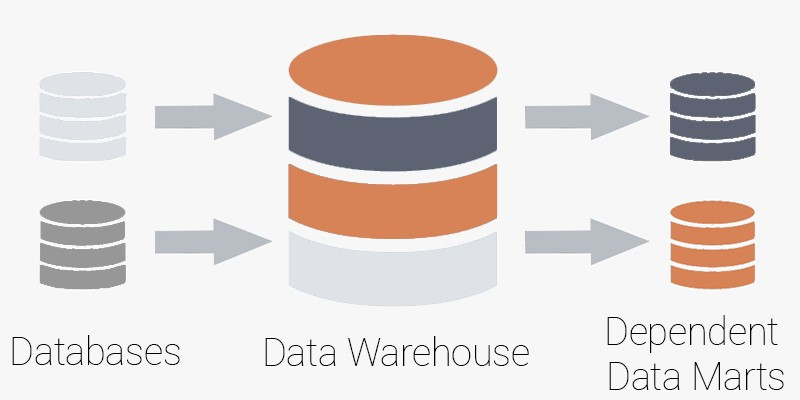
\includegraphics[width=15cm]{./IMAGENES/fiorella1}
				\end{center}
			\end{figure}

\subsection{DATA LAKE}

Data Lake es un término cuya primera definición o uso se atribuye a James Dixon que decía, “if you think of a datamart as akin to a bottle of water…”cleansed, packaged and structured for easy consumption” the data lake is more like a body of water in its natural state. Data flows from the streams (the source systems) to the lake. Users have access to the lake to examine, take samples or dive in.”

Sus principales funciones son  la gestión de la ingesta de datos, su almacenamiento y procesado posterior y, por último, el acceso a los mismos.

Algunas de sus características son:

\begin{itemize}
	
\item Contiene todos los datos de las fuentes originales, sin rechazar ningún tipo de dato.
\item Los datos se almacenan sin transformar o apenas transformados.
\item Los datos se transforman y se aplica un esquema sólo para satisfacer las necesidades de análisis.

\end{itemize}

\begin{figure}[htb]
				\begin{center}
					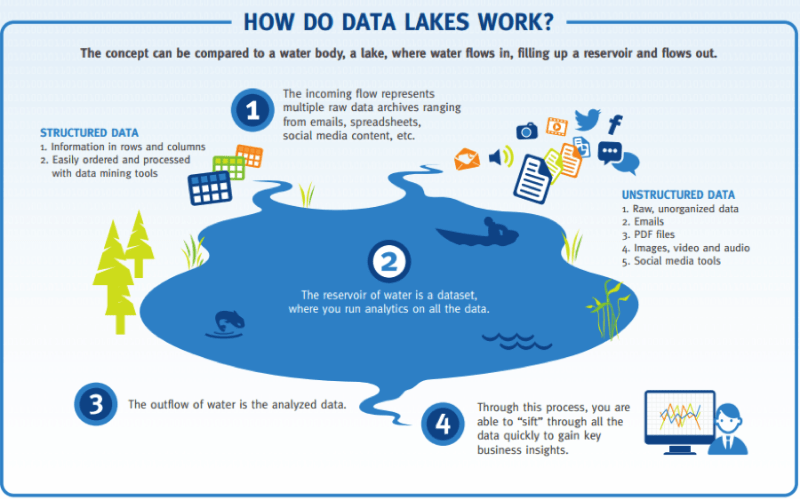
\includegraphics[width=15cm]{./IMAGENES/fiorella2}
				\end{center}
			\end{figure}

Es importante saber que al igual que cuando hablamos de Data Warehouse, por detrás hay una solución que soporta el modelo (Teradata, Oracle Exadata, SAP Hana, Microsoft SQL Server…) y muy habitualmente detrás de un Data Lake lo que está es la infraestructura del sistema de archivos HDFS (Hadoop Distributed File System) que utiliza Hadoop, y cuando hablamos de Hadoop en entornos corporativos generalmente hablamos de alguna de sus soluciones comerciales tales como Cloudera, Hortonworks, MapR, IBM o Pivotal, las 5 opciones más destacadas actualmente.

Tras las definiciones anteriores creo que es fácil resaltar alguna de las principales diferencias entre ambos conceptos

\begin{figure}[htb]
				\begin{center}
					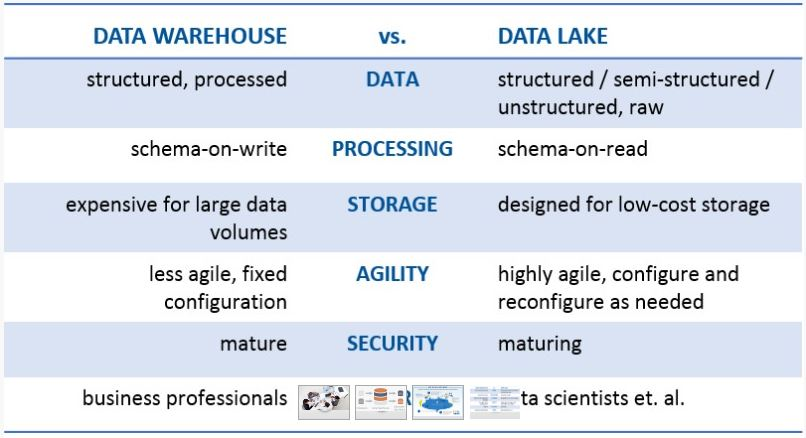
\includegraphics[width=15cm]{./IMAGENES/fiorella3}
				\end{center}
			\end{figure}
En definitiva es importante saber que aun siendo ambos conceptos, Data Warehouse y Data Lake, repositorios de información, un Data Lake no es una nueva versión 2.0 de un Data Warehouse ni su remplazo.

De hecho, se pueden complementar muy bien, diseñando una arquitectura de datos moderna, que permita seguir a las organizaciones aprovechando sus inversiones en su Data Warehouse, mientras que empiezan a recoger en su Data Lake, todos los datos que han sido ignorados o desechados anteriormente.


\subsection{DATA LAKE VS DATA WAREHOUSE}
	
Las divergencias entre Data Lake vs Data Warehouse pueden entenderse mejor repasando algunos de los puntos diferenciadores clave de un lago de datos y el modo en que contrastan con el enfoque del almacén de datos. Se trata de los siguientes:\\

\begin{itemize}

\item El lago de datos conserva todos los datos, a diferencia del almacén de datos, donde se dedica una parte importante de tiempo a decidir qué datos incluir y no incluir en el almacén
\item Un Data Lake admite todos los tipos de datos, independientemente de su tipo, formato o procedencia y sin necesidad de normalizar su estructura. La información se mantiene en su forma original y solo se transforma cuando se va a consumir.
\item El Data Lake puede nutrir a todos los usuarios de la organización, incluyendo a esos perfiles técnicos con exigencias de análisis más avanzadas, que son quienes recurren a capacidades como análisis estadístico y modelado predictivo.
\item A diferencia del Data Warehouse, el Data Lakes se adapta fácilmente a los cambios. El diseño del almacén es un proceso complejo y, la actualidad de loso negocios, en ocasiones no puede esperar tanto tiempo. Para esas circunstancias, asegura la adaptabilidad necesaria para entregar respuestas más rápidas.\\
\end{itemize}

Debido a que los lagos de datos contienen todos los datos y tipos de datos, y dado que permite a los usuarios acceder a los datos antes de que se hayan transformado, depurado y estructurado, también hace posible que se obtengan resultados más rápido de lo que sería posible con un enfoque tradicional de almacenamiento de datos.

Tanto los data lakes como los almacenes de datos se utilizan de forma generalizada para almacenar big data, pero no son términos intercambiables. Un data lake es un enorme conjunto de datos en bruto cuya finalidad no se ha definido todavía. Un almacén de datos es un repositorio de datos filtrados y estructurados que ya han sido procesados para una finalidad concreta.

La gente suele confundir estos dos tipos de almacenamiento de datos, cuando en realidad son mayores sus diferencias que sus semejanzas. A decir verdad, la única similaridad real entre ambos es su máxima finalidad, que es almacenar datos.

La diferencia es importante, porque están pensadas para objetivos distintos y exigen perspectivas diferentes para optimizarlas correctamente. Mientras que a una empresa le convendrá más tener un data lake, para otra resultará más oportuno disponer de un almacén de datos.


\begin{itemize}

\item Cuatro diferencias principales entre un data lake y un almacén de datos
\end{itemize}

Existen varias diferencias entre un data lake y un almacén de datos. Los principales diferenciadores son la estructura de los datos, los usuarios ideales, los métodos de procesamiento y la finalidad general de los datos.

\begin{figure}[htb]
				\begin{center}
					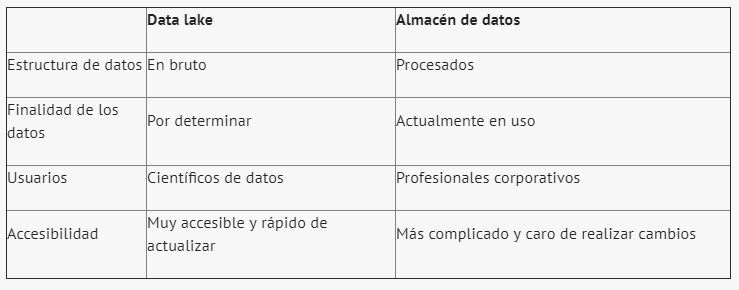
\includegraphics[width=15cm]{./IMAGENES/fiorella4}
				\end{center}
			\end{figure}

\begin{itemize}

\item Estructura de datos: En bruto frente a procesados

Los datos en bruto son datos que no aún no han sido procesados para ninguna finalidad. Quizá la principal diferencia entre los data lakes y los almacenes de datos sea la diversa estructura existente entre los datos en bruto y los procesados. En líneas generales un data lake almacena datos en bruto, sin procesar, mientras que un almacén guarda datos procesados y refinados.

Por ese motivo los data lakes suelen necesitar capacidades de almacenamiento mucho mayores que los almacenes de datos. Además, los datos en bruto, sin procesar, son maleables, pueden analizarse rápidamente a cualquier efecto y son idóneos para el machine learning. El riesgo de los datos en bruto, sin embargo, es que en ocasiones estos "lagos" que son los data lakes se convierten en pantanos de datos sin la presencia de la calidad de datos y las medidas de gobernanza adecuadas.

Los almacenes de datos, como tan solo guardan datos procesados, ahorran en espacio de almacenamiento, que es un recurso caro, porque no tienen que mantener datos que quizá nunca vayan a utilizarse. Además, los datos procesados los puede entender fácilmente un público más amplio.

\item Finalidad: Indeterminada o en uso

La finalidad de los componentes de datos individuales de un data lake no está establecida. Los datos en bruto se incorporan a un data lake, a veces con un uso futuro prefigurado y otras tan solo para tenerlos a mano. Esto significa que los data lakes presentan una menor organización y menor filtrado de sus datos que su equivalente.

Los datos procesados son datos en bruto a los que se ha asignado un uso concreto. Dado que los almacenes de datos tan solo albergan datos procesados, todos los datos de cualquier almacén de datos han sido utilizados para una finalidad específica dentro de la organización. Esto implica que el espacio de almacenamiento no se desperdicia en datos para los que puede que no se encuentre jamás una utilidad.

\item Usuarios: Científicos de datos frente a profesionales corporativos

Para un usuario que no esté familiarizado con los datos sin procesar, los data lakes son entornos en los que cuesta orientarse. Para entender los datos en bruto no estructurados y traducirlos a una aplicación comercial específica, se necesita ser un científico de datos y contar con herramientas especializadas.

De lo contrario, cada vez son más habituales las herramientas de preparación de datos que generan un acceso en autoservicio a la información almacenada en los data lakes.

Los datos procesados se emplean en gráficos, hojas de cálculo, tablas y demás representaciones para que la inmensa mayoría de los empleados de una empresa pueda consultarlos. Los datos procesados, al igual que los que encontramos en los almacenes de datos, tan solo exigen que el usuario tenga conocimientos de la temática representada.

\item Accesibilidad: Flexible frente a seguro

La accesibilidad y la facilidad de uso se refieren al uso del repositorio de datos en su totalidad, no a los datos que contiene. Los data lakes no tienen estructura y, por consiguiente, resulta fácil acceder a ellos y modificarlos. Además, cualquier cambio de los datos puede efectuarse rápidamente, dado que los data lakes tienen muy pocas limitaciones.

Por diseño, los almacenes de datos son más estructurados. Una de las ventajas más destacadas de los almacenes de datos es que el procesamiento y la estructura de los datos facilita su descodificación, pero las limitaciones de su estructura complican y encarecen su manipulación.

\end{itemize}

\subsection{DATA LAKE VS. DATA WAREHOUSE: PROBLEMA Y SOLUCION}	

\begin{itemize}

\item Problema

Ya estamos corriendo un gran almacén de datos para nuestro negocio, pero ahora la dirección quiere que construyamos un lago de datos. ¿Cual es la diferencia? ¿Dónde vamos a usarlo? ¿Quién va a usar?

\begin{figure}[htb]
				\begin{center}
					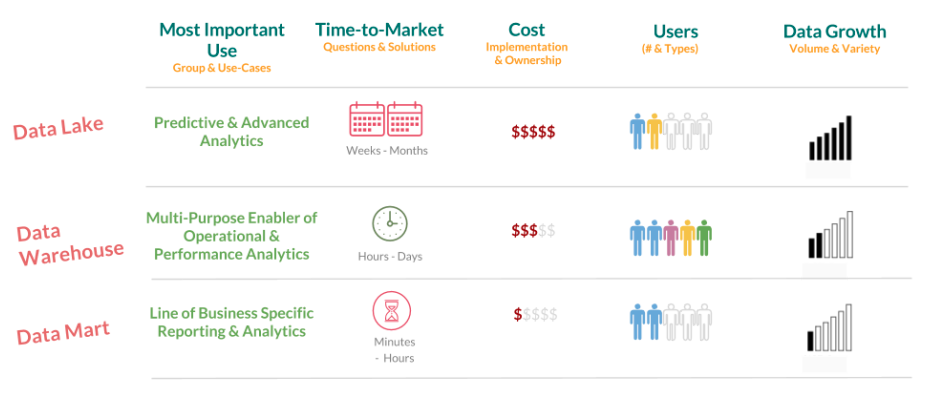
\includegraphics[width=15cm]{./IMAGENES/fiorella5}
				\end{center}
			\end{figure}

\item Solución

Un lago de datos es una ubicación centralizada para almacenar activos de datos de una organización en su forma nativa. Idealmente, estos activos de datos se recogen de todos los puntos de contacto del negocio y se almacenan con la intención de analizar en el futuro. El propósito de la captura de todos los elementos de datos de interés es asegurar que las empresas pueden utilizar para obtener una ventaja competitiva de mercado. Desde el inicio de la informática moderna, las bases de datos se han utilizado para este propósito. lagos de datos son una extensión natural de bases de datos - y almacenes de datos posteriores - en base a la variedad de datos y cómo se almacena o se utiliza.

de dejar que un decir una empresa decide capturar información acerca de sus interacciones con el cliente. Este ha sido el papel de CRM (Customer Relationship Management) aplicaciones durante mucho tiempo. Los usuarios registrarían de ventas potenciales, la retroalimentación del cliente y otra información en una base de datos CRM. Típicamente, la base de datos sería relacional con tablas predefinidas que representan al cliente y entidades asociadas.

Las empresas modernas interactúan con los clientes de muchas maneras diferentes sin embargo: puede haber un centro de llamadas de ladrillo y mortero utilizando un CRM; pero entonces habrá uno o más sitios web con sus formularios de comentarios, correos electrónicos directos, tienda de comercio electrónico, aplicaciones móviles, presencia en medios sociales o canales de socios de negocios. Todos estos son valiosas fuentes de información que pueden proporcionar una visión 360 del cliente. Para mantener una ventaja competitiva en el mercado, la empresa tendrá que capturar información de todos estos puntos de venta.

Pero no todas las piezas de información se puede guardar en una base de datos. Algunos datos serían muy poco estructuradas, como las imágenes (piensa en los usuarios que envían imágenes de productos defectuosos); algunos pueden ser semi-estructuradas, como las redes sociales se alimenta o documentos XML. Es imposible para almacenar todo tipo de datos en una sola base de datos y es ahí donde un lago de datos puede ayudar.

En su forma más básica, un lago de datos no es más que una enorme piscina de almacenamiento donde los datos pueden ser guardados en su forma nativa, sin procesar , sin ninguna transformación aplicada. Por ejemplo, un lago de datos puede almacenar ambas tandas nocturnas de archivos CSV (que se estructura de datos) descargadas desde el CRM y el streaming se alimenta desde el canal de medios sociales. El mismo lago de datos podría ser el hospedaje de archivos de la encuesta de satisfacción del cliente semi-estructurados enviados por terceros proveedores.

\end{itemize}


\subsection{SECCION 3}	


\subsection{SECCION 4}	


\section{Conclusion}
\begin{itemize}
\item Conclusion 1 : \\

\item Conclusion 2 : \\

\item Conclusion 3 : \\



\end{itemize}
%%
	
	%%
	%\linenumbers
	
	%% main text

	
	\newpage
	
	\bibliographystyle{apalike} 	%ESTILO
	\bibliography{BIBLIOGRAFIA}	 
\citep{DLake01}  
\citep{DLake02}  
\citep{DWarehouse01}  
\citep{DWarehouse02}  
\citep{DWarehouse03}  
\citep{DWarehouse03}  
\citep{DWarehouseVsDLake01}  
\citep{DWarehouseVsDLake02}  
	
%ARCHIVO .bib
	
	%% The Appendices part is started with the command \appendix;
	%% appendix sections are then done as normal sections
	%% \appendix
	
	%% \section{}
	%% \label{}
	
	%% References
	%%
	%% Following citation commands can be used in the body text:
	%% Usage of \cite is as follows:
	%%   \cite{key}          ==>>  [#]
	%%   \cite[chap. 2]{key} ==>>  [#, chap. 2]
	%%   \citet{key}         ==>>  Author [#]
	
	%% References with bibTeX database:
	
	
	%% Authors are advised to submit their bibtex database files. They are
	%% requested to list a bibtex style file in the manuscript if they do
	%% not want to use model1-num-names.bst.
	
	%% References without bibTeX database:
	
	% \begin{thebibliography}{00}
	
	%% \bibitem must have the following form:
	%%   \bibitem{key}...
	%%
	
	% \bibitem{}
	
	% \end{thebibliography}
	
\end{document}

%%
%% End of file `elsarticle-template-1-num.tex'.
